\PassOptionsToPackage{english}{babel}
\documentclass{report}
\usepackage[utf8]{inputenc}

%\usepackage[english]{babel}
%\usepackage[latin1]{inputenc}
%\usepackage{geometry}
%\usepackage{listings}
\usepackage{caption}
\usepackage{amsmath}
\usepackage{graphics}
\usepackage[T1]{fontenc}
\usepackage{enumitem} %bold enumeration
\usepackage[utf8]{inputenc}
\usepackage[english]{babel}
%\usepackage{pmgraph}
\usepackage{mathrsfs}
\usepackage{floatflt}
\usepackage{multicol}
\usepackage{color,colortbl}
% \usepackage[pdftex]{graphicx}
\usepackage[normalem]{ulem}
\usepackage[colorlinks,urlcolor=blue, linkcolor=blue]{hyperref}
\usepackage{epstopdf}
\usepackage{wrapfig}
\usepackage{multirow}
%% Sets page size and margins
\usepackage[a4paper,top=3cm,bottom=2cm,left=3cm,right=3cm,marginparwidth=1.75cm]{geometry}
%% Useful packages
\usepackage[colorinlistoftodos]{todonotes}
\usepackage{xymtex}
\usepackage{fancyhdr}
\usepackage{epstopdf}
\usepackage{indentfirst} \geometry{verbose,a4paper,tmargin=3cm,bmargin=3cm,lmargin=1.0cm,rmargin=2.0cm}
\setlength{\parindent}{0pt}
 \graphicspath{C:/Users/Anton/Desktop/ETH_books/CV/CV-Lab-Model-Fitting/CV-Lab-Model-Fitting/src/epipolar_geometry/res}
\begin{document}
\large
Report of Anton Maksimov (antonma, 16-952-137), Task 8 "Shape Context"\\
 on ETHZ course "Computer Vision".\\
\rule{\linewidth}{1pt}
%%%%%%%%%%%%%%%%%%%%%%%%%%%%%%%%%%%%%%%%%%%%%%%%%%%%%%%%%   1
	\textbf{1.} To compute shape descriptors we tried different strategies varying on method to assign angular component of the descriptor (flags to change mode are in the section of parameters in \texttt{shape\_matching.m}).  Suppose we have current point with position $p$ and we processing at the moment point at the distance between $r = $ \texttt{smallest\_r} and $R = $ \texttt{biggest\_r} distances. We calculate squared distance and place it in correspondent bin in between 
	\begin{enumerate}
		\item <<local>> --- angle as $\arctan$ of angle between $p1-p$ and X--axis. Problem is that it isn't rotationally invariant, so works well only when sets of points are not rotated initially.
		\item <<global>> --- we find difference of angles of $p1-c$ and $p-c$, where c is the center of the point cloud $(\max + \min)/2$ for both coordinates. Also isn't rotationally invariant and could work better for complex structures that the <<local>>.
		\item <<tangent>> --- we find the closest point $p_c$ to $p$, so get tangent angle $\tau$ as angle between $p_c-p$ and X axis. Then we calculate angles as in <<local>> mode, but subtracting $\tau$. As sampling is more or less uniform (when sample many enough points), the tangent direction could be well approximated with $p_c-p$.
	\end{enumerate}
\textbf{Problems with <<tangent>> mode.}
In paper attached to the task it's mentioned that for rotation--invariant descriptor it's better to use local system, such that calculate angles relatively to tangent direction. But it isn't said how to choose direction from two. We decided to calculate cost in the <<tangent>> mode such that we take the minimum value of two: when one descriptor is normal and when it's inverted with respect to angle values (if number of angular bins is even, it will mean that we changed direction tangent direction by $\pi/2$).


Another problem is that many figures are symmetric (hearts, forks are also), so points which are symmetric could be easily assigned to the opposite side and the figure will bend much, especially when number of iteration is big. So we used 3 iterations. After that it's clearly seen that parts which were assigned to the right side are fit well, though parts with incorrect side assignment try to bend more and more with every new iteration (fig. 1).

Also because of this bending we have to assign bigger $\lambda=10\cdot\text{mean\_distance}^2$ for smoothing. We don't change number of bins and rescaled $r$ and $R$, because they shouldn't depend on image in reality a priori (or we should use some automatic assignment of them).\\
\textbf{Conclusion}
In general, without removing outliers <<tangent>> mode works worse (+ because of the symmetry), but if remove outliers it should be better. It could be possible to use <<dummy>> points in template, which have some threshold level of cost for all points in image which we are trying to warp.
	\begin{figure}[h]
		\begin{center}
			\label{tang1}
			\begin{minipage}[h]{0.31\linewidth}
				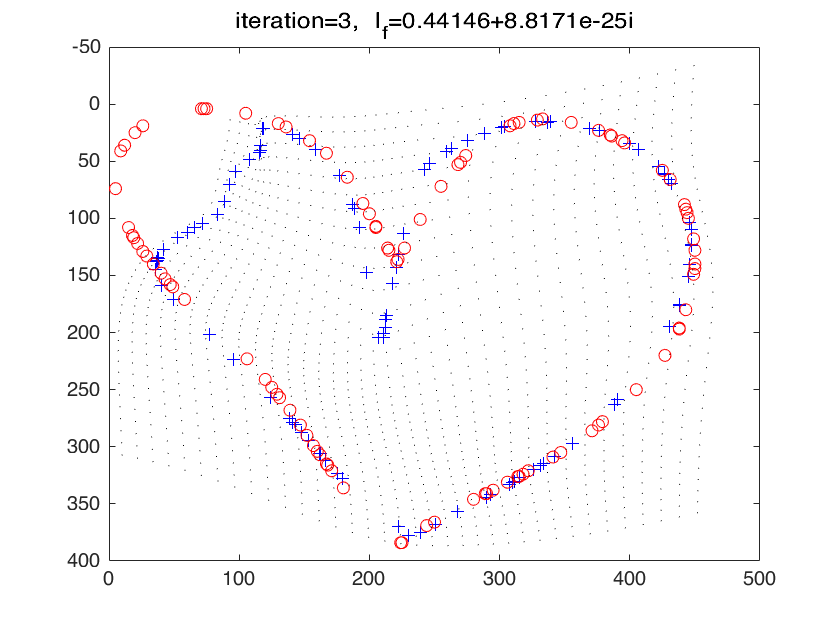
\includegraphics[width=1\linewidth, trim = {2cm 1cm 2cm 0cm}, clip]{C:/Users/Anton/Desktop/ETH_books/CV/cv_lab08_specific_recognition/code_release/results/12_tang1}
			\end{minipage}
			\hfill
			\begin{minipage}[h]{0.31\linewidth}
				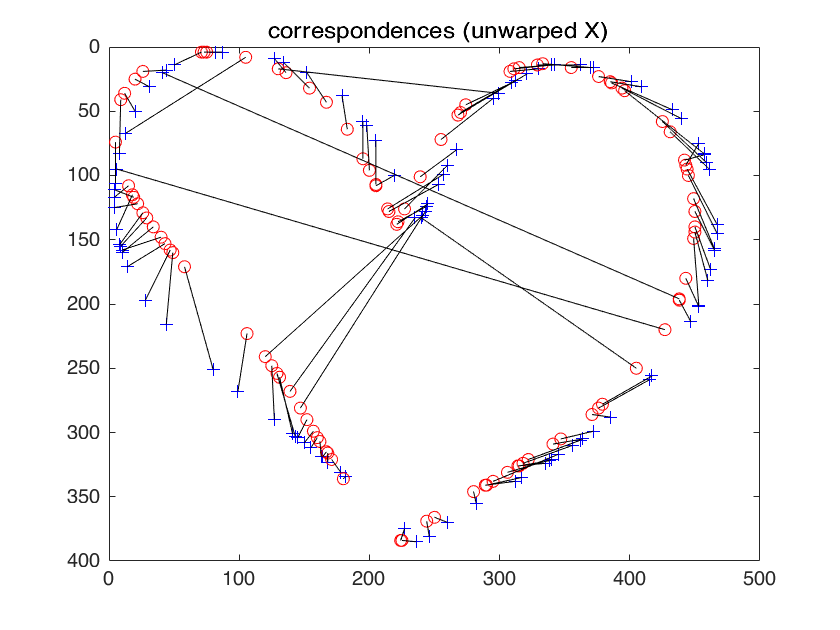
\includegraphics[width=1\linewidth, trim = {2cm 1cm 2cm 0cm}, clip]{C:/Users/Anton/Desktop/ETH_books/CV/cv_lab08_specific_recognition/code_release/results/12_tang2}
			\end{minipage}
				\hfill
				\begin{minipage}[h]{0.31\linewidth}
					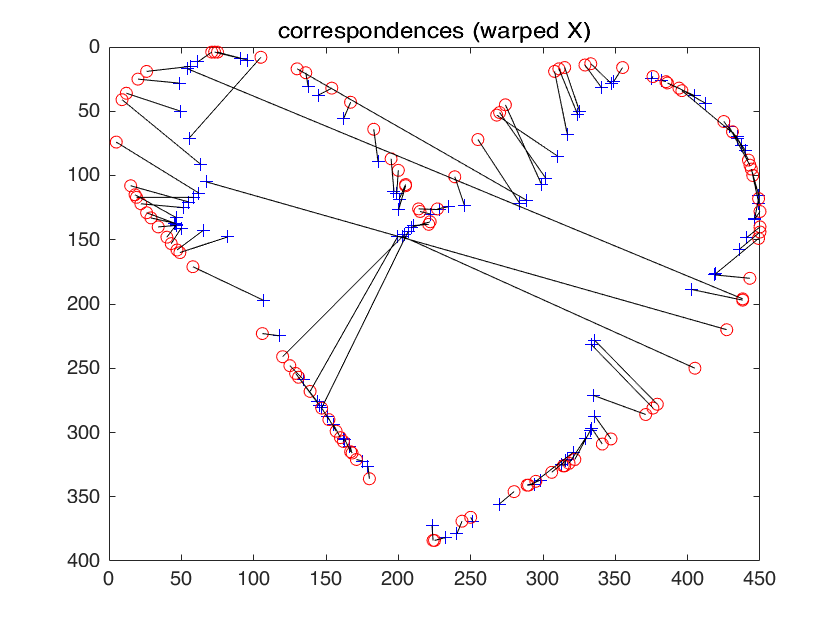
\includegraphics[width=1\linewidth, trim = {2cm 1cm 2cm 0cm}, clip]{C:/Users/Anton/Desktop/ETH_books/CV/cv_lab08_specific_recognition/code_release/results/12_tang3}
				\end{minipage}
			
		\caption{<<Tangent>> mode, $\lambda=10\cdot\text{mean\_distance}^2$, 3 iterations.}
	\end{center}
\end{figure}

	\begin{figure}[h]
	\begin{center}
		\label{tang1}
		\begin{minipage}[h]{0.31\linewidth}
			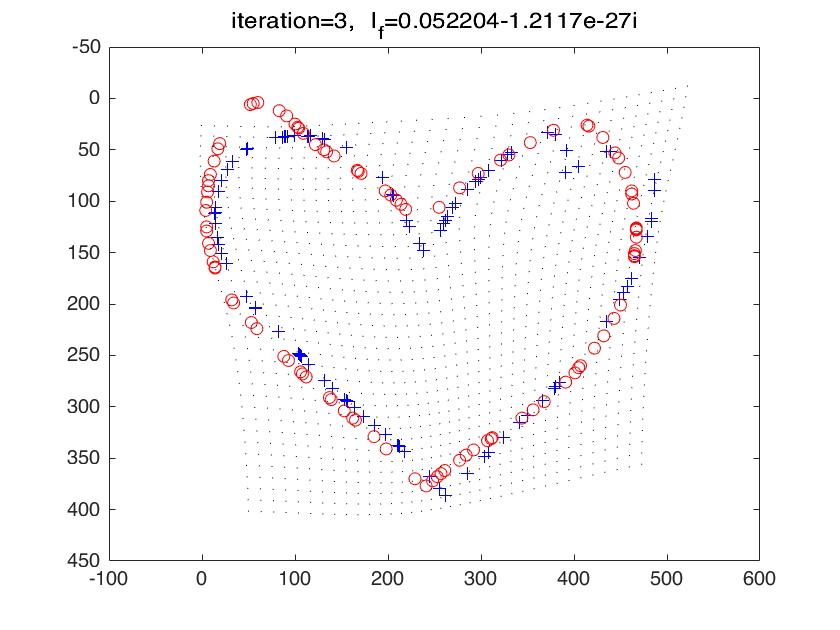
\includegraphics[width=1\linewidth, trim = {2cm 1cm 2cm 0cm}, clip]{C:/Users/Anton/Desktop/ETH_books/CV/cv_lab08_specific_recognition/code_release/results/34_local2}
		\end{minipage}
		\hfill
		\begin{minipage}[h]{0.31\linewidth}
			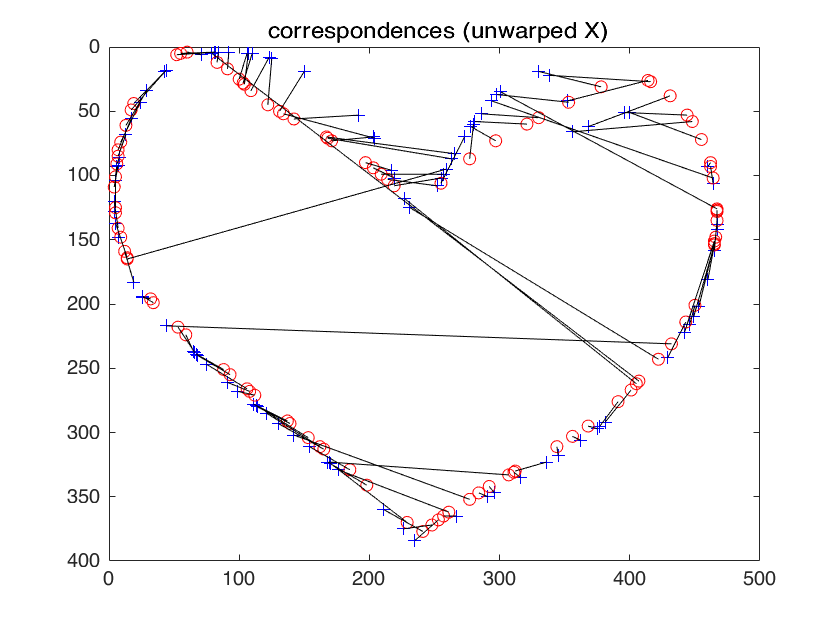
\includegraphics[width=1\linewidth, trim = {2cm 1cm 2cm 0cm}, clip]{C:/Users/Anton/Desktop/ETH_books/CV/cv_lab08_specific_recognition/code_release/results/34_local1}
		\end{minipage}
		\hfill
		\begin{minipage}[h]{0.31\linewidth}
			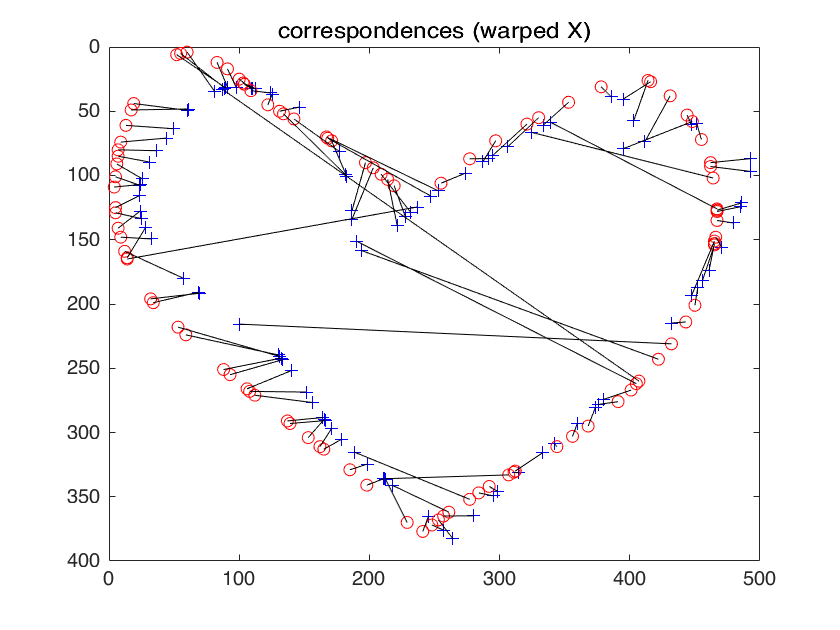
\includegraphics[width=1\linewidth, trim = {2cm 0cm 2cm 0cm}, clip]{C:/Users/Anton/Desktop/ETH_books/CV/cv_lab08_specific_recognition/code_release/results/34_local3}
		\end{minipage}
		
		\caption{<<Local>> mode, $\lambda=10\cdot\text{mean\_distance}^2$, 3 iterations.}
	\end{center}
\end{figure}


\begin{figure}[h]
	\begin{center}
		\label{tang1}
		\begin{minipage}[h]{0.31\linewidth}
			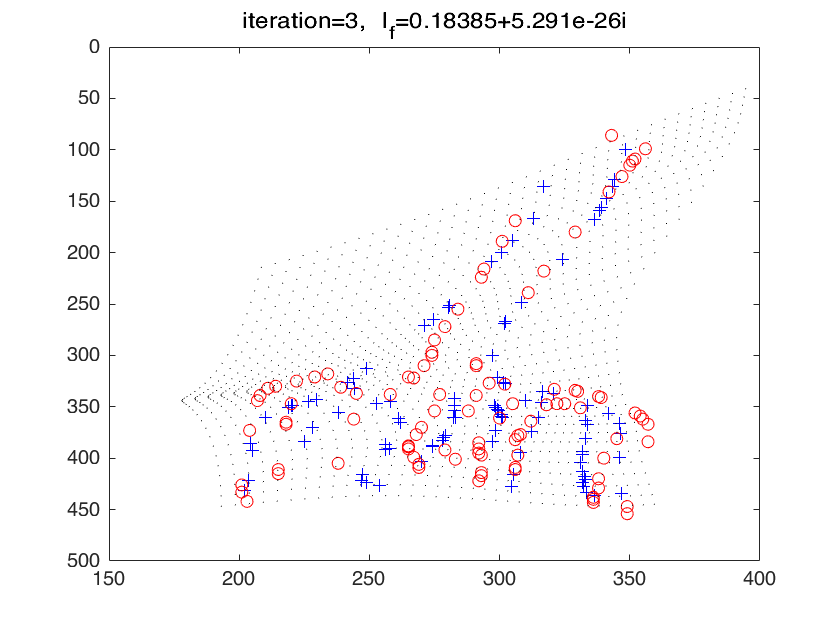
\includegraphics[width=1\linewidth, trim = {2cm 1cm 2cm 0cm}, clip]{C:/Users/Anton/Desktop/ETH_books/CV/cv_lab08_specific_recognition/code_release/results/67_local1}
		\end{minipage}
		\hfill
		\begin{minipage}[h]{0.31\linewidth}
			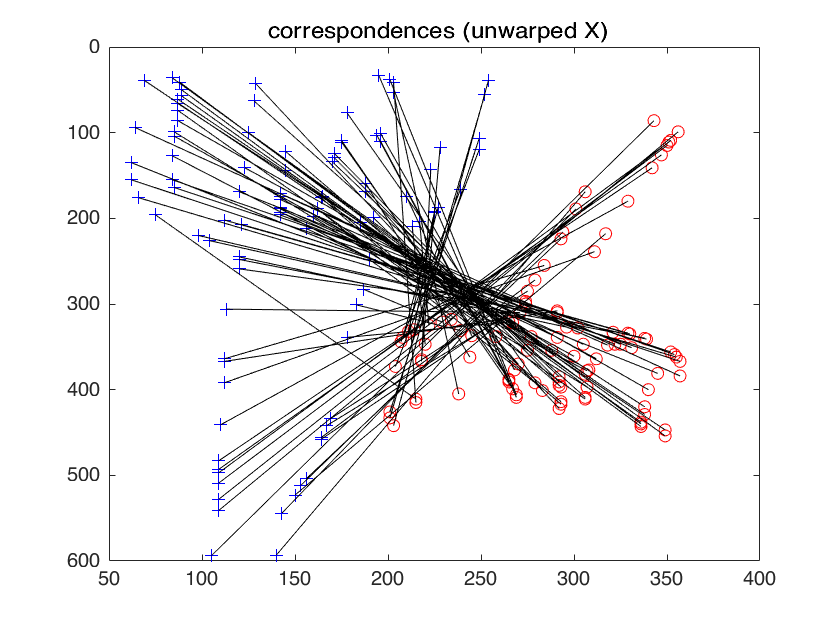
\includegraphics[width=1\linewidth, trim = {2cm 1cm 2cm 0cm}, clip]{C:/Users/Anton/Desktop/ETH_books/CV/cv_lab08_specific_recognition/code_release/results/67_local2}
		\end{minipage}
		\hfill
		\begin{minipage}[h]{0.31\linewidth}
			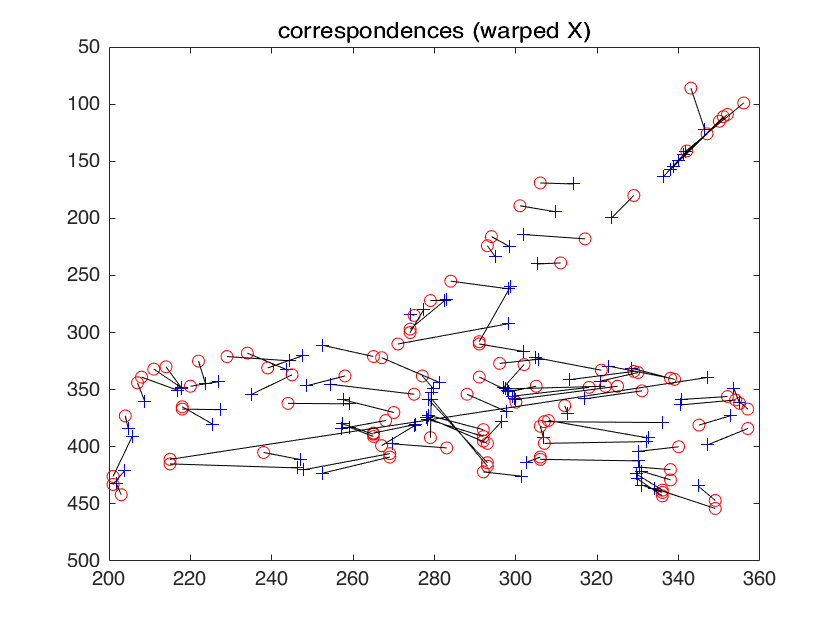
\includegraphics[width=1\linewidth, trim = {2cm 1cm 2cm 0cm}, clip]{C:/Users/Anton/Desktop/ETH_books/CV/cv_lab08_specific_recognition/code_release/results/67_local3}
		\end{minipage}
		
		\caption{<<Local>> mode, $\lambda=10\cdot\text{mean\_distance}^2$, 3 iterations.}
	\end{center}
\end{figure}


\begin{figure}[h]
	\begin{center}
		\label{tang1}
		\begin{minipage}[h]{0.31\linewidth}
			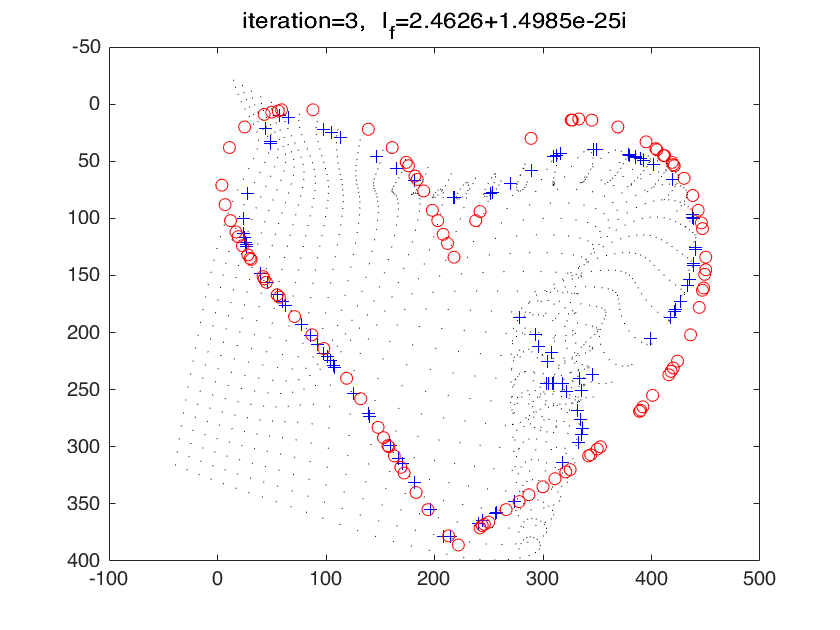
\includegraphics[width=1\linewidth, trim = {2cm 1cm 2cm 0cm}, clip]{C:/Users/Anton/Desktop/ETH_books/CV/cv_lab08_specific_recognition/code_release/results/12_glob1}
		\end{minipage}
		\hfill
		\begin{minipage}[h]{0.31\linewidth}
			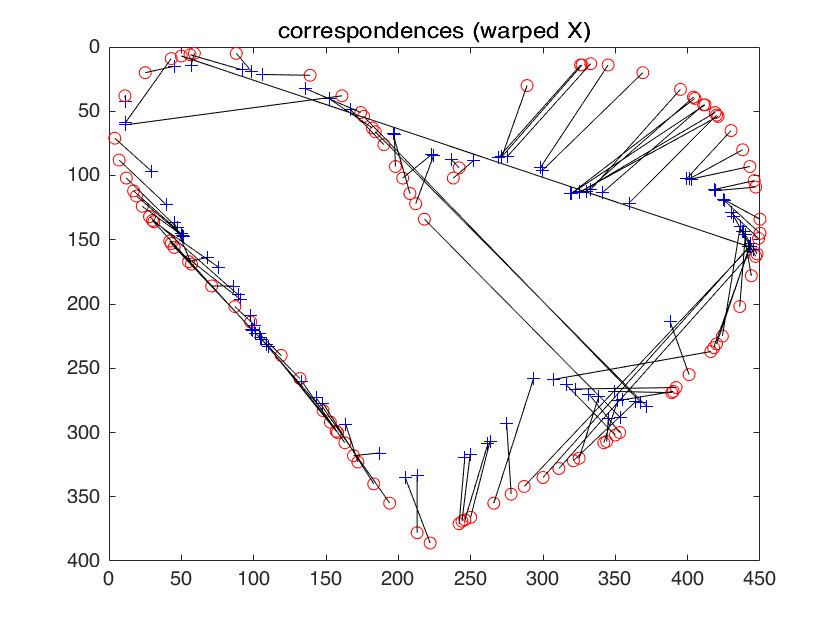
\includegraphics[width=1\linewidth, trim = {2cm 1cm 2cm 0cm}, clip]{C:/Users/Anton/Desktop/ETH_books/CV/cv_lab08_specific_recognition/code_release/results/12_glob2}
		\end{minipage}
		\hfill
		\begin{minipage}[h]{0.31\linewidth}
			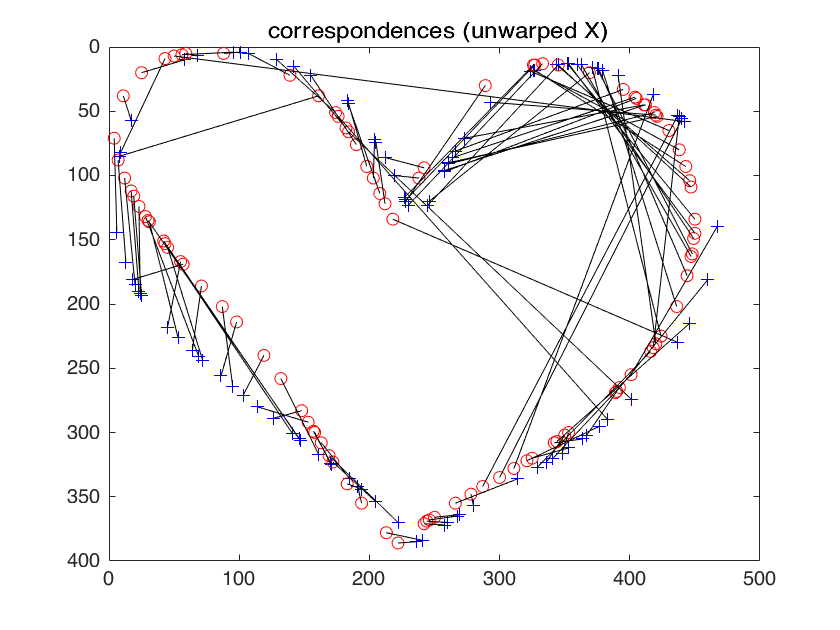
\includegraphics[width=1\linewidth, trim = {2cm 0cm 2cm 0cm}, clip]{C:/Users/Anton/Desktop/ETH_books/CV/cv_lab08_specific_recognition/code_release/results/12_glob3}
		\end{minipage}
		
		\caption{<<Global>> mode, $\lambda=10\cdot\text{mean\_distance}^2$, 3 iterations.}
	\end{center}
\end{figure}
%%%%%%%%%%%%%%%%%%%%%%%%%%%%%%%%%%%%%%%%%%%%%%%%%%%%%%%%%%%%%%%%%%
\newpage
\textbf{Answer to question.}
Yes, shape--context descriptors are scale--invariant (all three modes we mentioned in the beginning), because they use points as the origin of local coordinate system and distances are normalized using mean distance between points, which scales equally with distances between selected point and others.
\end{document}